\subsection{Work Activities}
	\subsubsection{Software Requirement Specification}
	\begin{itemize}
		\item SRS-T001: SRS Draft
		\begin{itemize}
			\item SRS-T001-1: Brainstorming meeting for ideas.
			\item SRS-T001-2: Understand and develop user requirement.
			\item SRS-T001-3: Define product features and functional requirement.
			\item SRS-T001-4: Develop external interface and non-functional requirements.
			\item SRS-T001-5: SRS draft finalization meeting.
		\end{itemize}
		\item SRS-T002: SRS Final Version
		\begin{itemize}
			\item  SRS-T002-1: Revise SRS draft following client's recommendations after SRS draft presentation meeting.
			\item  SRS-T002-2: Keep track client requirements change every weeks.
			\item  SRS-T002-3: Team review meeting before release official SRS document.
		\end{itemize}
	\end{itemize}

	\subsubsection{Software Product Management Plan}
	\begin{itemize}
		\item SPMP-T001: SPMP Draft
		\begin{itemize}
			\item SPMP-T001-1: Brainstorming meeting for ideas.
			\item SPMP-T001-2: Develop project organization, specific role and responsibility for each member in this project.
			\item SPMP-T001-3: Develop risk management plan.
			\item SPMP-T001-4: Analysis team characteristics and select appropriate process model.  
			\item SPMP-T001-5: Create working plan based on current SRS, process model and team capacity.
			\item SPMP-T001-6: SPMP draft finalization meeting.
		\end{itemize}
		\item SPMP-T002: SPMP Final Version
		\begin{itemize}
			\item  SPMP-T002-1: Revise SPMP draft following client's recommendations after SPMP draft presentation meeting.
			\item  SPMP-T002-2: Weekly update if there is with any change in process model, resources, development plan etc.
			\item  SPMP-T002-3: Team review meeting before release official SPMP document.
		\end{itemize}
	\end{itemize}

	\subsubsection{Software Design Document}
	\begin{itemize}
			\item SDD-T001: System Design
			\begin{itemize}
				\item SDD-T001-1: Develop system overview of product.
				\item SDD-T001-2: Define system components base on system overview.
				\item SDD-T001-3: System components design details for each component
			\end{itemize}
			\item SDD-T002: GUI Design
			\begin{itemize}
				\item SDD-T002-1: Analyst user requirements and system features.
				\item SDD-T002-2: Define GUI appropriate with each features.
				\item SDD-T002-3: Create the mock-GUI and test it feasibility and user experience.
			\end{itemize}
			\item SDD-T003: SDD Final Version
			\begin{itemize}
				\item  SDD-T003-1: Revise SDD draft following client's recommendations after SDD draft presentation meeting.
				\item  SDD-T003-2: Weekly update if there is with any change in requirements, features which need to be reflect into system design, GUI design etc.
				\item  SDD-T003-3: Team review meeting before release official SDD document.
			\end{itemize}
	\end{itemize}

	\subsubsection{Implementation}
	\begin{itemize}
		\item IMP-T001: Prototyping
		\begin{itemize}
				\item IMP-T001-1: Create simple manual control with UI.				
				\item IMP-T001-2: Create autonomous controller make robot move randomly with human control.
				\item IMP-T001-3: Enhance from IM-T001-2 make robot move follow a track to test color sensor.
				\item IMP-T001-4: Enhance from IM-T001-2 make robot automatically moving while detect and avoid obstacle. 
		\end{itemize}
		\item IMP-T002: GUI Implementation
		\begin{itemize}
				\item IMP-T002-1: Create GUI from mock-up design of SDD-T002.
				\item IMP-T002-2: Integration prototyping with new GUI.
				\item IMP-T002-3: Implement user input feature on GUI. Allow user to manually add new information such as NGZ, destination, landing site etc.
		\end{itemize}
		\item IMP-T003: Implement autonomous mode.
		\begin{itemize}
				\item IMP-T003-1: Implement path finding algorithm.
				\item IMP-T003-2: Enhance IMP-T001-3 and IMP-T001-4 so that robot can recognize and follow the track.
				\item IMP-T003-3: Enhance IMP-T001-3 and IMP-T001-4 so that robot can recognize physical obstacle, NGZ, cratters etc. 
				\item IMP-T003-3: Implement area map survey strategy by moving zig-zag while detect and avoid obstacles, NGZ, cratters etc.
		\end{itemize}
		\item IMP-T004: Implement manual control mode.
		\begin{itemize}
				\item IMP-T004-1: Implement warning and confirmation when user control robot into danger region.
				\item IMP-T004-2: Implement emergency stop feature.
				\item IMP-T004-3: Implement autonomous/manual switch.
		\end{itemize}
		\item IMP-T005: Map Display and Construction.
		\begin{itemize}
			\item IMP-T005-1: Display import map xml info onto GUI-MAP.
			\item IMP-T005-2: Display new informations return from sensor on GUI-MAP.
			\item IMP-T005-3: Display warning on GUI-MAP when robot move into danger region.
			\item IMP-T005-4: Implement export result survey xml map.
		\end{itemize}
		\item IMP-T006: Team final review.
		\begin{itemize}
			\item IMP-T006-1: Each member review all implemented features.
			\item IMP-T006-2: Final review meeting and collect team features feedback.
			\item IMP-T006-3: Make change base on feedback.
		\end{itemize}
	\end{itemize}

	\subsubsection{Testing}
	\begin{itemize}
		\item Test-T001: Unit Test.
		\begin{itemize}
				\item Test-T001-1: Create unit test for all major computation component.
				\item Test-T001-2: Regular review and make test case up to date.
		\end{itemize}
		\item Test-T002: Integration Test.
		\begin{itemize}
				\item Test-T002-1: Define test cases and test-acceptance criteria base on requirement and scope define in SRS.
				\item Test-T002-2: Meeting with client and finalize all test cases.
				\item Test-T003-3: Perform test product functionalities base on defined test cases while implement process.
				\item Test-T003-4: Keep track all change in requirement and update corresponding test cases.
				\item Test-T003-5: Recording all fail tests and keep track along side with development process.
		\end{itemize}
	\end{itemize}

	\subsubsection{User Manual}
	\begin{itemize}
		\item UM-T001: Define user manual structure.
		\begin{itemize}
				\item UM-T001-1: Team brainstorming for user manual ideas.
				\item UM-T001-2: Create user manual draft.
				\item UM-T001-3: Present and get feedback from clients.
		\end{itemize}
		\item UM-T002: Finalize user manual. 
		\begin{itemize}
				\item UM-T001-1: Review client feedback and revise user manual.
				\item UM-T002-2: Team meeting and release final version.
		\end{itemize}
	\end{itemize}

	\subsubsection{Release}
	\begin{itemize}
		\item RL-T001: Pre-Relase
		\begin{itemize}
			\item RL-T001-1: Run over all test case define in Test-T001 and Test-T002.
			\item RL-T001-2: Review and check is there any existing bug.
			\item RL-T001-3: Fix all fail test cases and existing bug. 
		\end{itemize}
		\item RL-T002: Create review checklist.
		\item RL-T003: Go over release checklist and deploy final product to client.
	\end{itemize}
	
	
\subsection{Milestone}
	\subsubsection{Internal Milestone}
		\begin{itemize}
			\item IMS-001: Robot manual control with basic movement.
			\begin{itemize}
				\item Due Date: End of week 3.
				\item Description:
				\begin{itemize}
					\item Simple GUI with buttons : Up, Down, Left, Right, Stop.
					\item Robot move as expected when use control button on GUI.
				\end{itemize}
			\end{itemize}
			\item IMS-002: Software Requirement Specification Draft.
			\begin{itemize}
				\item Due Date: End of week 4.
				\item Description:
				\begin{itemize}
					\item Have first draft of SRS document follow SRS template with all sections in detail.
					\item Document must be in LaTEX file.
					\item Document manager must perform proof-reading over whole document and edit spelling, grammar, formating mistake if any.
				\end{itemize}
			\end{itemize}
			\item IMS-003: Software Project Management Plan Draft
			\begin{itemize}
				\item Due Date: End of week 6.
				\item Description:
				\begin{itemize}
					\item Have first draft of SPMP document follow SPMP template with all sections in detail.
					\item Document must be in LaTEX file.
					\item Document manager must perform proof-reading over whole document and edit spelling, grammar, formating mistake if any.
				\end{itemize}
			\end{itemize}
			\item IMS-004: Mock-up of final GUI
			\begin{itemize}
				\item Due Date: End of week 6.
				\item Description:
				\begin{itemize}
					\item Finish GUI design with all GUI component which user need to finish their mission.
					\item Go through SRS user requirement, system features make sure all requirement can perform easy on GUI.
					\item Some buttons, features or component on GUI may not working since it just placeholder. 
				\end{itemize}
			\end{itemize}
			\item IMS-005: Software Design Document Draft
			\begin{itemize}
				\item Due Date: End of week 8.
				\item Description:
				\begin{itemize}
					\item Have first draft of SPMP document follow SPMP template with all sections in detail.
					\item Document must be in LaTEX file.
					\item Document manager must perform proof-reading over whole document and edit spelling, grammar, formating mistake if any.
				\end{itemize}
			\end{itemize}
			\item IMS-006: Robot autonomous survey mode
			\begin{itemize}
				\item Due Date: End of week 9.
				\item Description:
				\begin{itemize}
					\item Robot can automatically move inside survey area.
					\item Robot can detect and avoid obstacle, cratter, NGZ and avoid them.
					\item Robot can collect sensor data and display it on GUI-Map.
					\item Robot can move to point define by user.
					\item Robot can move follow track.
				\end{itemize}
			\end{itemize}
			\item IMS-007: Finish final GUI functionalities
				\begin{itemize}
				\item Due Date: End of week 10.
				\item Description:
				\begin{itemize}
					\item Every function on GUI work as define in SDD user interface section.
				\end{itemize}
			\end{itemize}
			\item IMS-008: Integration and Testing
			\begin{itemize}
				\item Due Date: End of week 11.
				\item Description:
				\begin{itemize}
					\item Integrate manual control mode and autonomous mode in to GUI.
					\item Verify all functionalities still working as expected and match with requirement in SRS document.
					\item Switch between manual/autonomous without any problem.
					\item Robot can complete survey in less than 20 minutes and return to landing site.
				\end{itemize}
			\end{itemize}
			\item IMS-009: Prepare for final presentation with client.
			\begin{itemize}
				\item Due Date: End of week 12.
				\item Description:
				\begin{itemize}
					\item All remaining must be solve.
					\item All test case must pass.
					\item Code review already perform and have a clear code base with sufficient up to date comment.
					\item Final code must be submit before code freeze deadline.
					\item Slide or Postcard must ready if there is required them.
				\end{itemize}
			\end{itemize}
		\end{itemize}
	\subsubsection{Client Official Milestone}
		\begin{itemize}
			\item OMS-001: Client Official Milestone 1 Demo.
			\begin{itemize}
				\item Due Date: End of week 7.
				\item Description:
				\begin{itemize}
					\item Finish GUI design with all GUI components which user need to finish their mission.
					\item Robot movement display correct on Map-GUI.
					\item Robot can move randomly and avoid obstacles and NGZ.
					\item Some buttons, features or component on GUI may not working since it is just placeholder. 
				\end{itemize}
			\end{itemize}
			\item OMS-002 : Client Official Milestone 2 Demo.
			\begin{itemize}
				\item Due Date: End of semester break.
				\item Description:
				\begin{itemize}
					\item Robot can move survey the area with effective strategy such as move cycle or zig-zag.
					\item User can manual define NGZ and robot can recognize NGZ, obstacle, crater to avoid them while survey.
					\item New informations of survey area are display in real-time on GUI-Map.
				\end{itemize}
			\end{itemize}
		\end{itemize}
	
	\subsection{Work Breakdown Structure}
The Fig.\ref{work-breakdown-structure} shows a work breakdown structure of this project. This project consists of 5 difference phases: Verfication of requirement, Project management plan development, Software development, Testing and product release. 
	\begin{figure}[H]
		\centering
		\hspace*{-1.3in}
		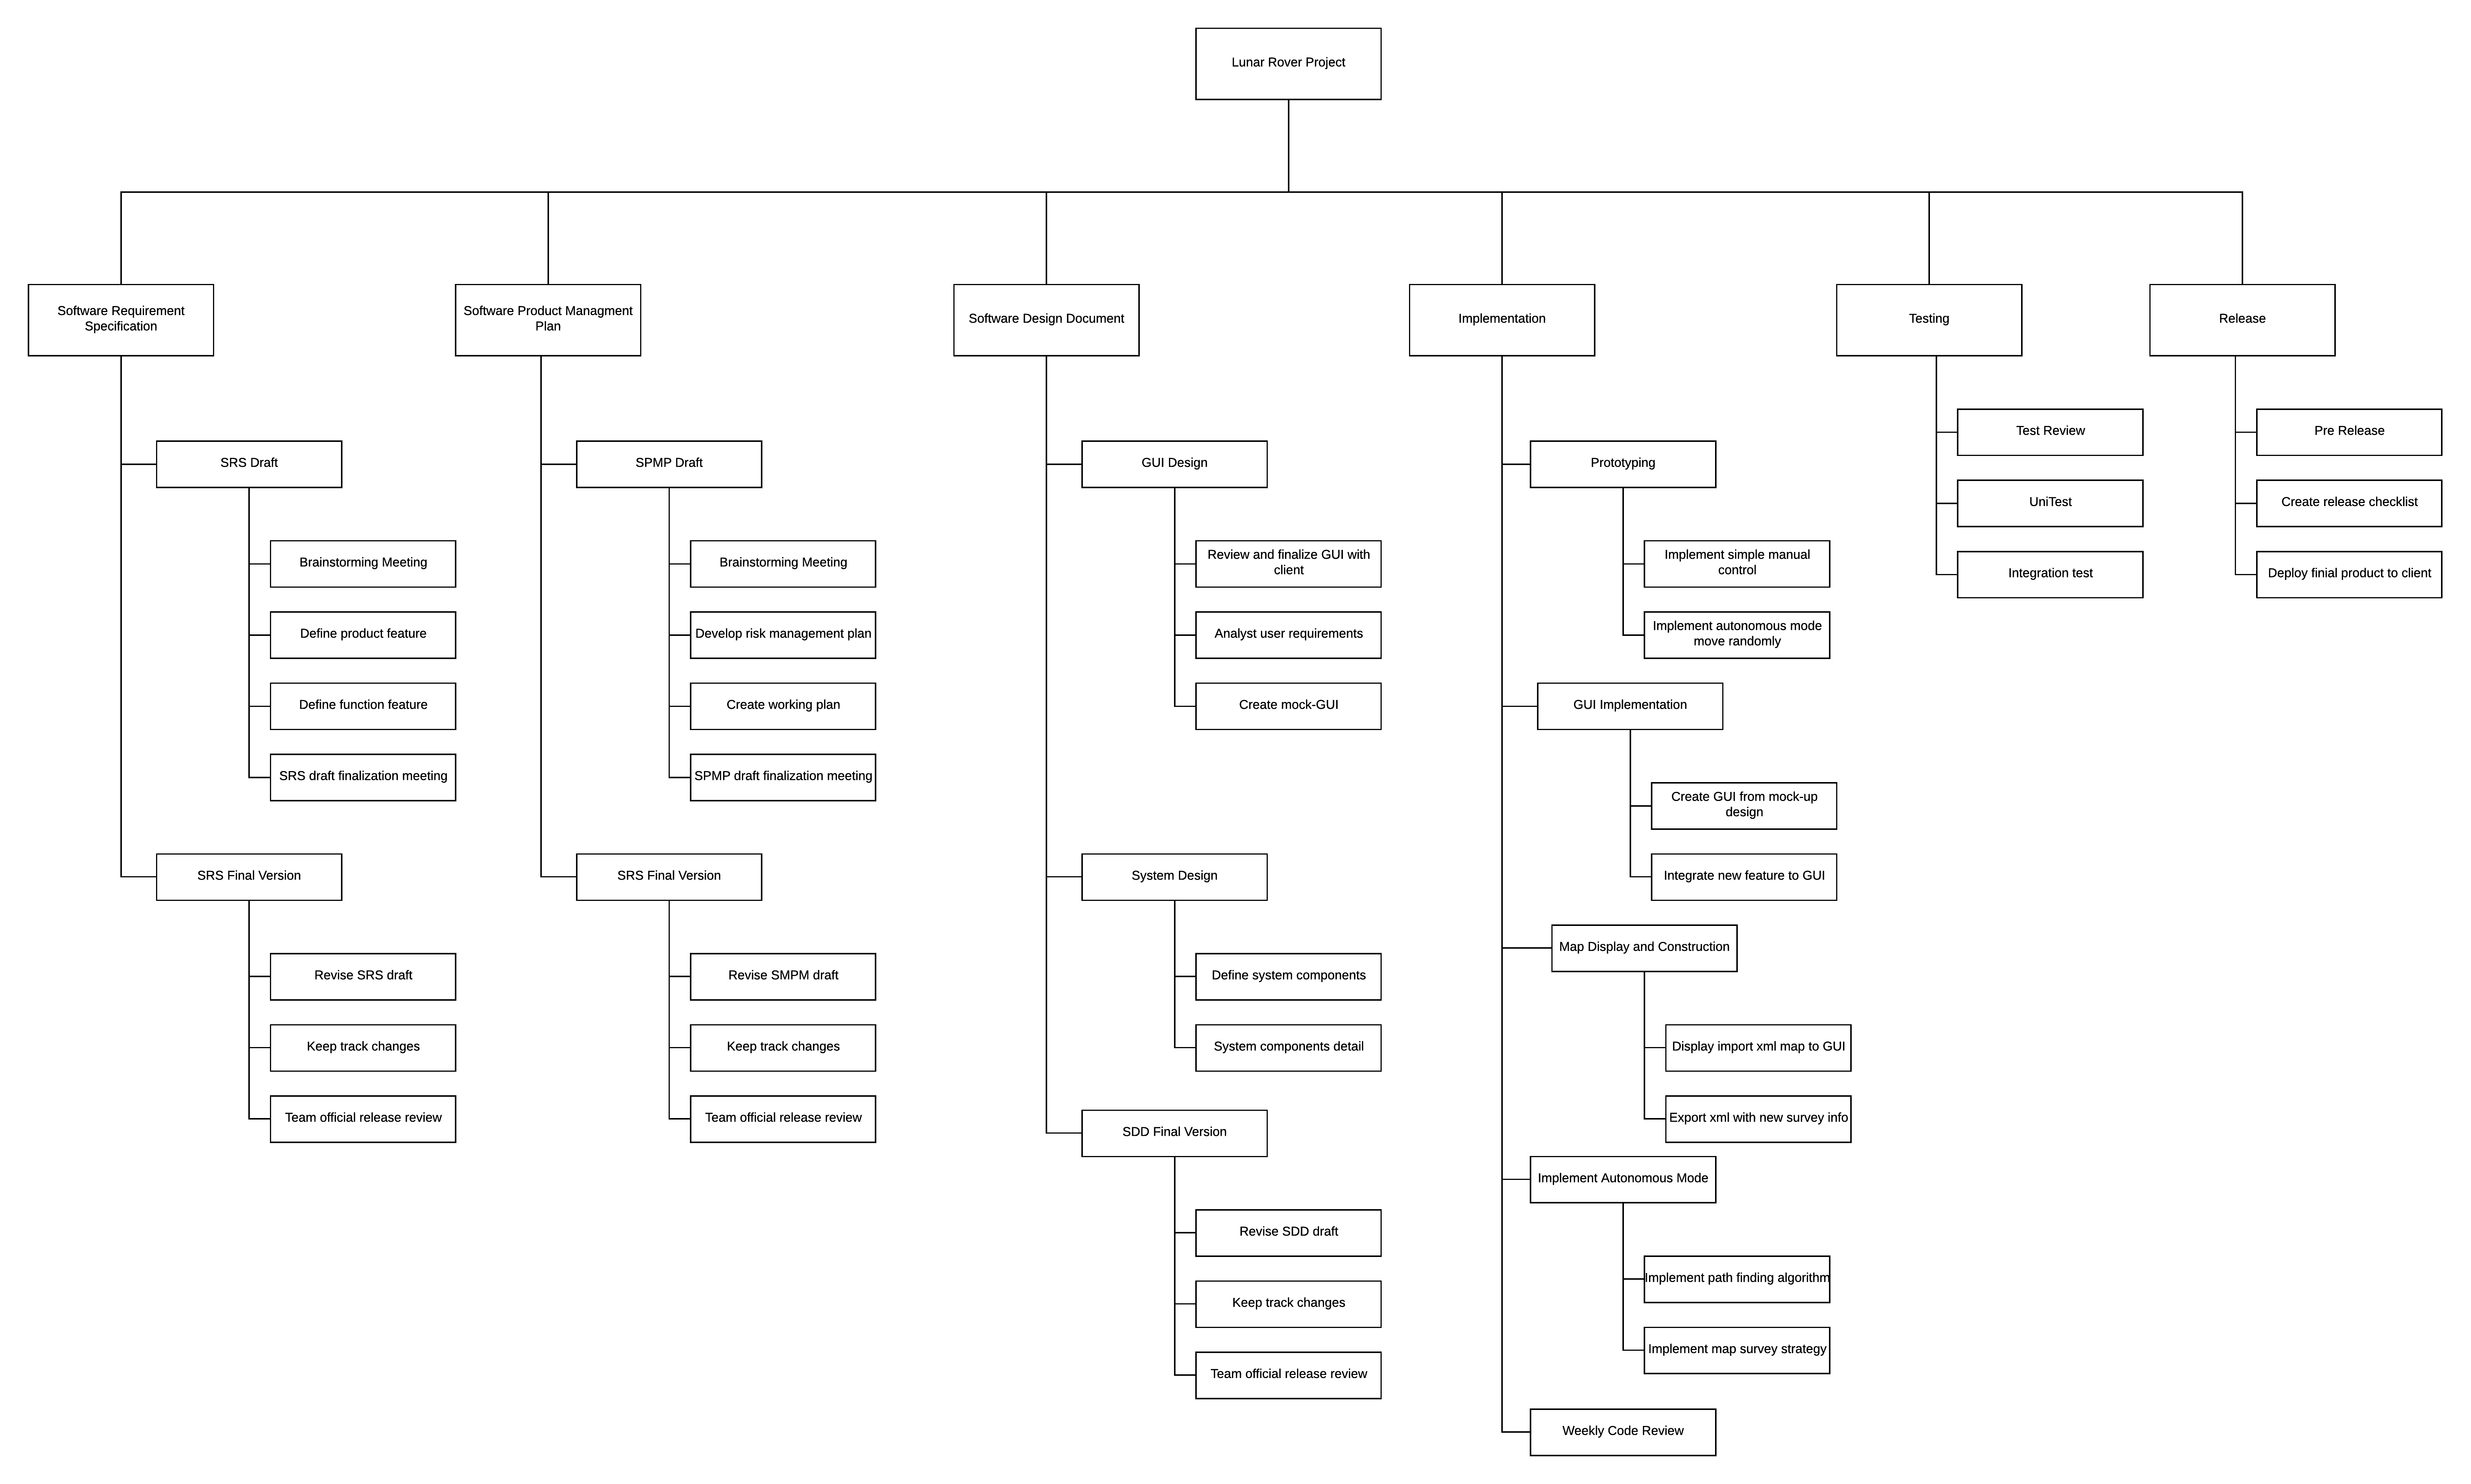
\includegraphics[width=1.5\linewidth]{WorkBreakDown_s.PNG}  % created using www.draw.io
		\caption{Work Breakdown Structure}
		\label{work-breakdown-structure}
	\end{figure}
\subsection{Schedule Allocation}
\subsubsection{Task schedule}
The task scheduling will be shown in detail by the Gantt chart below. In summary, the Gantt chart will indicate which team member has responsibility for a task. The time allocation for each task with a specific  deadline. Tasks can work in parallels are also visualize and can easy to find in the chart.     
\subsubsection{Major Task and Deadline Time}
	\begin{tabular}{|p{3cm}|p{8cm}|}
		\hline 
		\textbf{Deadline Time} &\textbf{Task name} \\ 
		\hline 
			Week 5 & Software Requirement Specification Draft\\ 
		\hline 
			Week 7 & Software Project Management Plan Draft\\ 
		\hline 		
			Week 7 & Milestone 1 demo specification finalize and sign agreement\\ 
		\hline 
			Week 8 & Milestone 1 demo\\ 
		\hline 
			Week 8 & Milestone 2 demo specification finalize and sign agreement\\ 
		\hline 
			Week 9 & Software Design Document Draft\\ 
		\hline 
			Week 9 & Milestone 2 demo\\ 
		\hline 		
			Week 11 & User manual and instruction draft\\ 
		\hline 
			Week 12 & Release final version of SRS, SPMP, SDD and user manual\\ 
		\hline 
			Week 12 & Code free and product release\\ 
		\hline 
	\end{tabular} 

